% Intended LaTeX compiler: pdflatex
\documentclass[letterpaper]{article}
\usepackage[utf8]{inputenc}
\usepackage[T1]{fontenc}
\usepackage{graphicx}
\usepackage{longtable}
\usepackage{wrapfig}
\usepackage{rotating}
\usepackage[normalem]{ulem}
\usepackage{amsmath}
\usepackage{amssymb}
\usepackage{capt-of}
\usepackage{hyperref}
\usepackage{lmodern} % Ensures we have the right font
\usepackage{listings} % Syntax highlighting
\usepackage{lmodern} % Ensures we have the right font
\usepackage[utf8]{inputenc}
\usepackage{graphicx}
\usepackage{amsmath, amsthm, amssymb}
\usepackage[table, xcdraw]{xcolor}
\date{}
\title{Resultados}
\hypersetup{
 pdfauthor={vian},
 pdftitle={Resultados},
 pdfkeywords={},
 pdfsubject={},
 pdfcreator={Emacs 28.2 (Org mode 9.5.5)}, 
 pdflang={Spanish}}
\begin{document}

\maketitle
\tableofcontents


\section{Notación}
\label{sec:org49a6e67}
\textbf{fun} = Mínimo local hallado de la función \emph{execute\textunderscore circuit} con el optimizador
\newline
\textbf{p} = Número de capas (a mayor número el circuito es más profundo)
\newline
\textbf{theta} = Lista de parámetros [\(\beta\)\textsubscript{1}, \ldots{}, \(\beta\)\textsubscript{p}, \(\gamma\)\textsubscript{1}, \ldots{}, \(\gamma\)\textsubscript{p}] del circuito cuántico
\newline
\textbf{num iterations} = Número de iteraciones del compilador necesarias para hallar el mínimo
\newline
\textbf{seed\textunderscore simulator} = Semilla utilizada en la ejecución del circuito para fijar la aleatoriedad en \emph{backend.run()}
\newline
\textbf{X\textsubscript{ij}} = Se refiere a la arista \textbf{i} -> \textbf{j}. 1 Si dicha arista es parte del camino resultante, 0 en otro caso
\newline
\textbf{q\textsubscript{n}} = Qubit enésimo
\newline
q\textsubscript{4}q\textsubscript{3}q\textsubscript{2}q\textsubscript{1}q\textsubscript{0} = X\textsubscript{23}X\textsubscript{13}X\textsubscript{12}X\textsubscript{02}X\textsubscript{01}
\newpage

\section{Primer grafo}
\label{sec:orgdb0025b}
\begin{center}
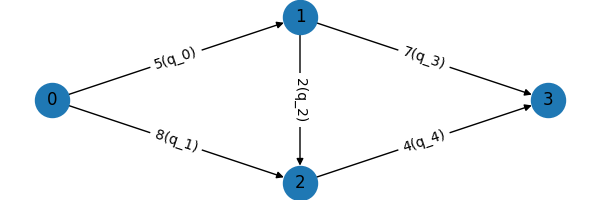
\includegraphics[width=.9\linewidth]{./img/primer_grafo.png}
\end{center}
\newpage
\subsection{Aer - Versión del paper (primer\textunderscore grafo/aer-qaoa.ipynb)}
\label{sec:org5b1c373}
Pruebas realizadas sobre la versión del código sin la restricción\newline
    \textbf{X\textsubscript{13} + X\textsubscript{23} = 1}\newline

Versión equivalente a la de [\href{https://www.mdpi.com/1424-8220/22/19/7570/xml}{Multi-Objective Routing Optimization for 6G Communication Networks Using a Quantum Approximate Optimization Algorithm-sensors-22-07570-v2}]

\begin{itemize}
\item \textbf{Estadísticas:}

Realizando la ejecución 1000 veces se han obtenido como caminos resultantes los siguientes:
\end{itemize}
\begin{center}
\begin{tabular}{|r|l|r|}
\hline
\textbf{Qubits} & \textbf{Camino} & \textbf{Frecuencia} (1000)\\
\hline
10101 & X\textsubscript{01}X\textsubscript{12}X\textsubscript{23} & 917\\
10110 & X\textsubscript{02}X\textsubscript{12}X\textsubscript{23} & 82\\
01001 & X\textsubscript{01}X\textsubscript{13} & 1\\
\hline
\end{tabular}
\end{center}
\newpage

\subsubsection{Caso correcto}
\label{sec:org2ff3d16}

\begin{center}
\begin{tabular}{|r|l|r|r|}
\hline
\textbf{fun} & \textbf{theta} & \textbf{num iterations} & \textbf{seed\textunderscore simulator}\\
\hline
29.63 & [0.7739, 0.9302] & 29 & 10\\
\hline
\end{tabular}
\end{center}

\begin{figure}[htbp]
\centering
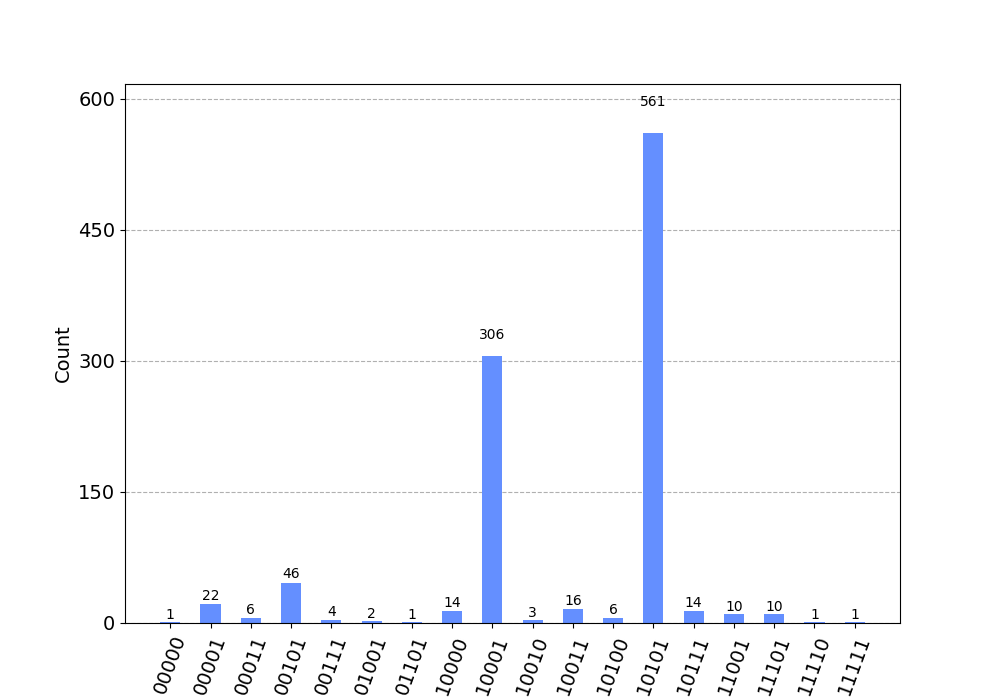
\includegraphics[scale=0.5]{./img/primer_paper_aer_correcto.png}
\caption{seed\textunderscore simulator=10}
\end{figure}

Mejor resultado: 10101 (q\textsubscript{4}q\textsubscript{3}q\textsubscript{2}q\textsubscript{1}q\textsubscript{0} = X\textsubscript{23}X\textsubscript{13}X\textsubscript{12}X\textsubscript{02}X\textsubscript{01})

Camino: X\textsubscript{01}X\textsubscript{12}X\textsubscript{23} (Camino óptimo)

\newpage

\subsubsection{Caso erróneo}
\label{sec:org2c3382c}

\begin{center}
\begin{tabular}{|r|l|r|r|}
\hline
\textbf{fun} & \textbf{theta} & \textbf{num iterations} & \textbf{seed\textunderscore simulator}\\
\hline
52.79 & [0.6320  0.7177] & 35 & 21\\
\hline
\end{tabular}
\end{center}

\begin{figure}[htbp]
\centering
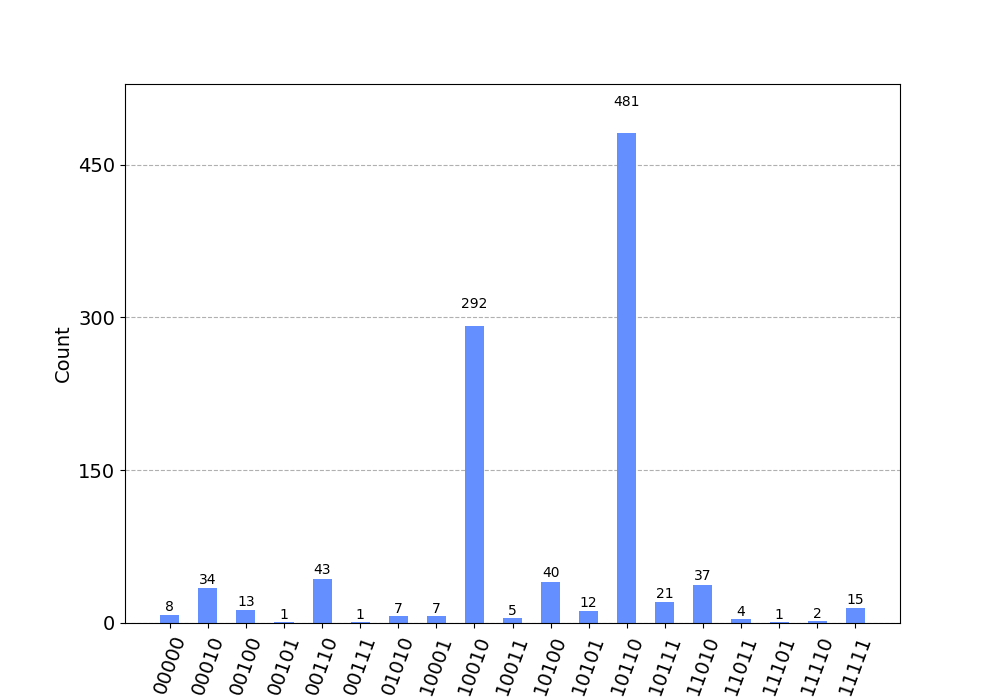
\includegraphics[scale=0.5]{./img/primer_paper_aer_erroneo.png}
\caption{seed\textunderscore simulator=21}
\end{figure}

Mejor resultado: 10110 (q\textsubscript{4}q\textsubscript{3}q\textsubscript{2}q\textsubscript{1}q\textsubscript{0} = X\textsubscript{23}X\textsubscript{13}X\textsubscript{12}X\textsubscript{02}X\textsubscript{01})

Camino: X\textsubscript{02}X\textsubscript{12}X\textsubscript{23} (Camino incorrecto. Rompe 2 restricciones)

Restricciones rotas: \newline
    \textbf{X\textsubscript{02}+X\textsubscript{12}=X\textsubscript{23}} \newline
    \textbf{X\textsubscript{01}=X\textsubscript{12}+X\textsubscript{13}} \newline

\newpage

\subsubsection{Caso subóptimo}
\label{sec:org56f36b1}

Obtenido a mano (no se ha encontrado ninguna semilla que diese este resultado)

\begin{center}
\begin{tabular}{|r|l|}
\hline
\textbf{fun} & \textbf{theta}\\
\hline
67.33 & [-0.4811, 1.566]\\
\hline
\end{tabular}
\end{center}

\begin{center}
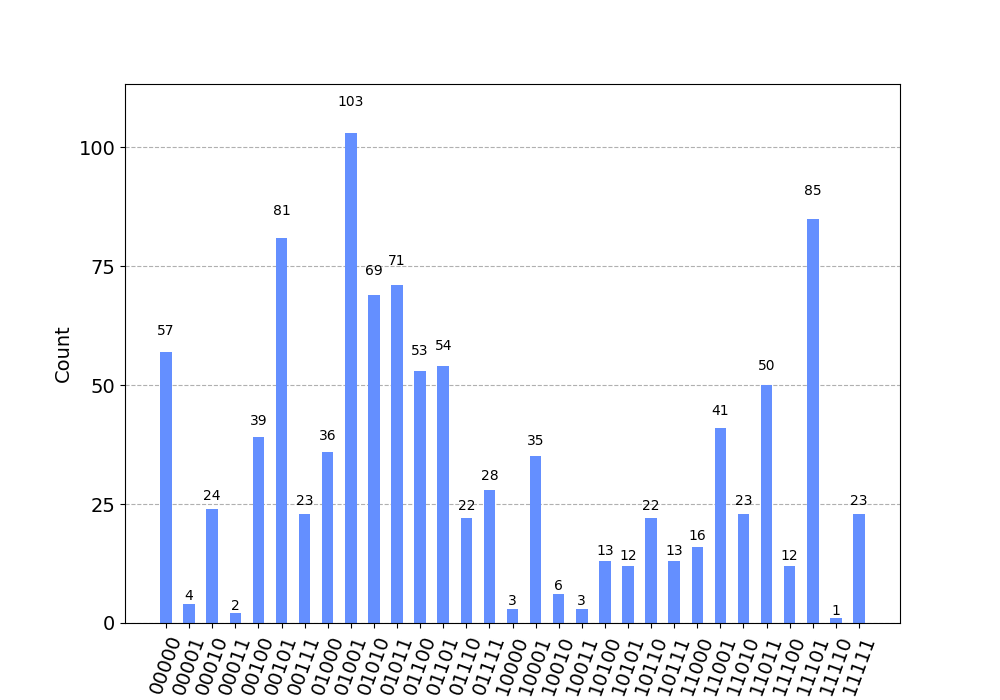
\includegraphics[scale=0.5]{./img/primer_paper_aer_suboptimo.png}
\end{center}

Mejor resultado: 01001 (q\textsubscript{4}q\textsubscript{3}q\textsubscript{2}q\textsubscript{1}q\textsubscript{0} = X\textsubscript{23}X\textsubscript{13}X\textsubscript{12}X\textsubscript{02}X\textsubscript{01})

Camino: X\textsubscript{01}X\textsubscript{13} (Camino subóptimo, pero no se rompe ninguna restricción)

\newpage

\subsubsection{Utilizando el parámetro \textbf{theta} obtenido en el artículo}
\label{sec:org995b779}

\begin{center}
\begin{tabular}{|r|l|}
\hline
\textbf{fun} & \textbf{theta}\\
\hline
65.40 & [0.28517317, -5.05969577]\\
\hline
\end{tabular}
\end{center}

\begin{center}
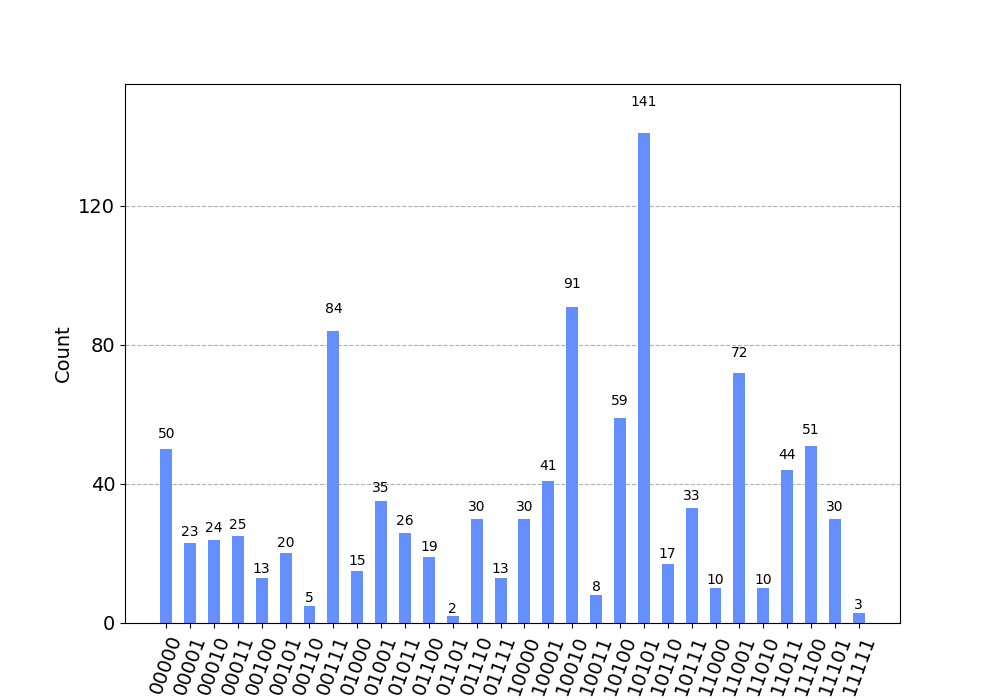
\includegraphics[scale=0.5]{./img/primer_paper_aer_resultado.png}
\end{center}

Mejor resultado: 10101 (q\textsubscript{4}q\textsubscript{3}q\textsubscript{2}q\textsubscript{1}q\textsubscript{0} = X\textsubscript{23}X\textsubscript{13}X\textsubscript{12}X\textsubscript{02}X\textsubscript{01})

Camino: X\textsubscript{01}X\textsubscript{12}X\textsubscript{23} (Camino óptimo)

La gráfica resultante es muy similar a la versión que se intenta replicar. \textbf{fun} tiene resultados muy altos, entre 65 y 70 (en comparación con la versión del código con la restricción extra).

\newpage

\subsection{Aer simulator con restricción extra  (primer\textunderscore grafo/con\textunderscore restricc/aer-qaoa.ipynb)}
\label{sec:org29963ac}
Con respecto a la función de coste del paper se añade la restricción\newline
    \textbf{X\textsubscript{13} + X\textsubscript{23} = 1}\newline
Esto sería, que el camino solo llegue al nodo final \textbf{3} por una de las aristas X\textsubscript{i3} existentes.

\begin{itemize}
\item \textbf{Estadísticas:}
\end{itemize}

Realizando la ejecución 1000 veces se han obtenido como caminos resultantes los siguientes:

\begin{center}
\begin{tabular}{|r|l|r|}
\hline
\textbf{Qubits} & \textbf{Camino} & \textbf{Frecuencia (1000)}\\
\hline
10101 & X\textsubscript{01}X\textsubscript{12}X\textsubscript{23} & 938\\
11000 & X\textsubscript{13}X\textsubscript{23} & 37\\
10001 & X\textsubscript{01}X\textsubscript{23} & 9\\
00011 & X\textsubscript{01}X\textsubscript{02} & 11\\
00100 & X\textsubscript{12} & 3\\
00010 & X\textsubscript{02} & 1\\
11111 & X\textsubscript{01}X\textsubscript{02}X\textsubscript{12}X\textsubscript{13}X\textsubscript{23} & 1\\
\hline
\end{tabular}
\end{center}

\newpage

\subsubsection{Caso correcto}
\label{sec:org6dec763}
\begin{center}
\begin{tabular}{|r|l|r|r|}
\hline
\textbf{fun} & \textbf{theta} & \textbf{num iterations} & \textbf{seed\textunderscore simulator}\\
\hline
42.29 & [0.5081, 0.9401] & 33 & 3\\
\hline
\end{tabular}
\end{center}

\begin{figure}[htbp]
\centering
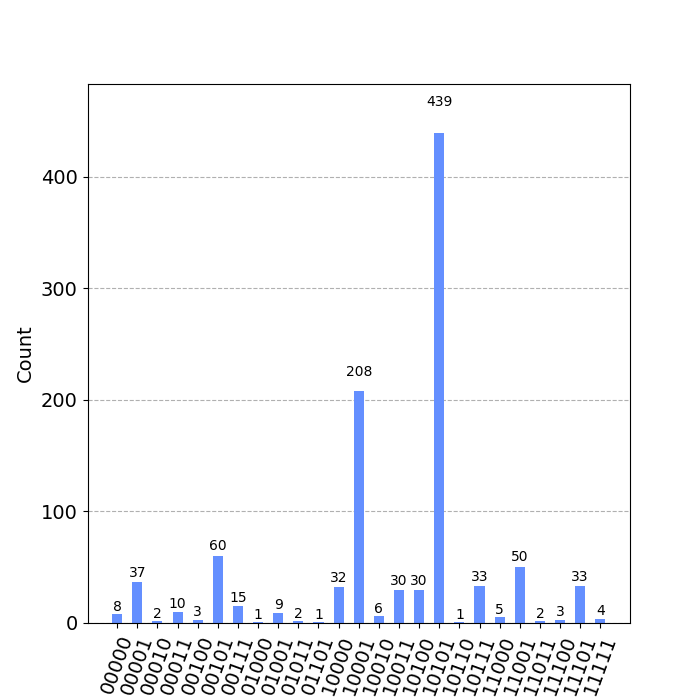
\includegraphics[scale=0.5]{./img/primer_restr_aer_correcto.png}
\caption{seed\textunderscore simulator=3}
\end{figure}

Mejor resultado: 10101 (q\textsubscript{4}q\textsubscript{3}q\textsubscript{2}q\textsubscript{1}q\textsubscript{0} = X\textsubscript{23}X\textsubscript{13}X\textsubscript{12}X\textsubscript{02}X\textsubscript{01})

Camino: X\textsubscript{01}X\textsubscript{12}X\textsubscript{23} (Camino óptimo)

\newpage

\subsubsection{Caso "correcto" con ruido}
\label{sec:org46fc634}
\begin{center}
\begin{tabular}{|r|l|r|r|}
\hline
\textbf{fun} & \textbf{theta} & \textbf{num iterations} & \textbf{seed\textunderscore simulator}\\
\hline
90.75 & [0.9962, 1.995] & 27 & 2\\
\hline
\end{tabular}
\end{center}

\begin{figure}[htbp]
\centering
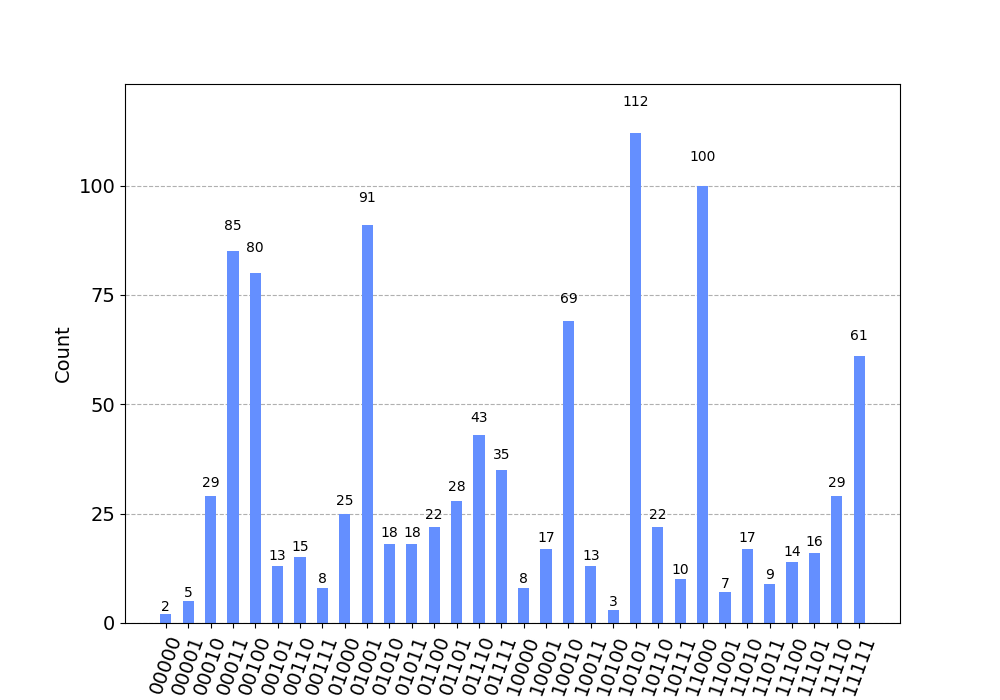
\includegraphics[scale=0.5]{./img/primer_restr_aer_correcto-con-ruido.png}
\caption{seed\textunderscore simulator=2}
\end{figure}

Mejor resultado: 10101 (q\textsubscript{4}q\textsubscript{3}q\textsubscript{2}q\textsubscript{1}q\textsubscript{0} = X\textsubscript{23}X\textsubscript{13}X\textsubscript{12}X\textsubscript{02}X\textsubscript{01})

Camino: X\textsubscript{01}X\textsubscript{12}X\textsubscript{23} (Camino óptimo)

Aunque se obtenga el resultado óptimo (10101) existen otros resultados demasiado altos, e incluso ejecutando el circuito con el mismo \textbf{theta} se dan valores distintos. Podría afectar a los resultados de las estadísticas.

Además se ve que encuentra un valor \textbf{fun} demasiado alto (90.75)

\newpage

\subsection{Provider}
\label{sec:org4dc6a18}
\begin{itemize}
\item ibmq\textunderscore lima
\end{itemize}
\begin{figure}[htbp]
\centering
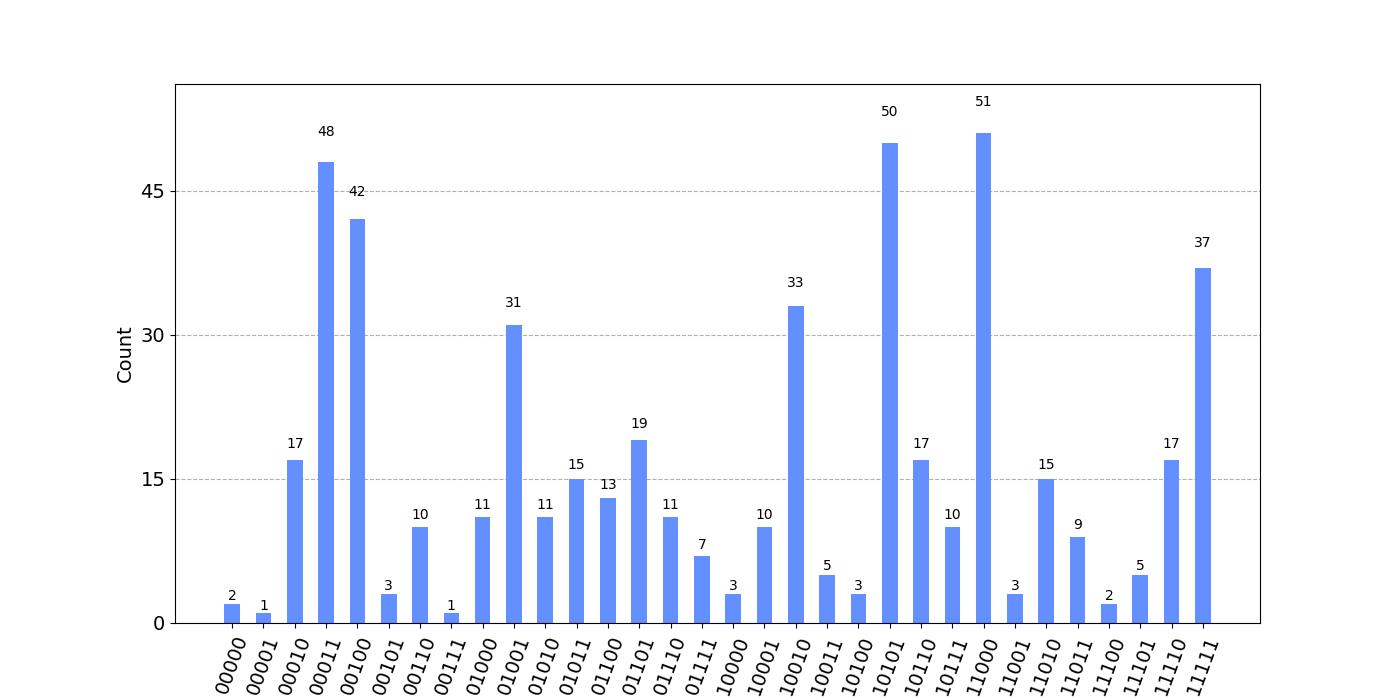
\includegraphics[scale=0.4]{./img/primer_provider_iter-2.png}
\caption{num iterations=2}
\end{figure}
Solo para comprobar que funciona la ejecución.
\end{document}